%%%% Proceedings format for most of ACM conferences (with the exceptions listed below) and all ICPS volumes.
\documentclass[sigconf]{acmart}
%%%% As of March 2017, [siggraph] is no longer used. Please use sigconf (above) for SIGGRAPH conferences.

%%%% Proceedings format for SIGPLAN conferences 
% \documentclass[sigplan, anonymous, review]{acmart}

%%%% Proceedings format for SIGCHI conferences
% \documentclass[sigchi, review]{acmart}

%%%% To use the SIGCHI extended abstract template, please visit
% https://www.overleaf.com/read/zzzfqvkmrfzn


\usepackage{booktabs} % For formal tables


% Copyright
% \setcopyright{none}
%\setcopyright{acmcopyright}
%\setcopyright{acmlicensed}
\setcopyright{rightsretained}
%\setcopyright{usgov}
%\setcopyright{usgovmixed}
%\setcopyright{cagov}
%\setcopyright{cagovmixed}


% DOI
\acmDOI{10.475/123_4}

% ISBN
\acmISBN{123-4567-24-567/08/06}

%Conference
\acmConference[DAC'19]{ Design Automation conference}{June 2019}{
  LasVegas, NV USA}
\acmYear{2019}
\copyrightyear{2019}


% These commands are optional
%\acmBooktitle{Transactions of the ACM Woodstock conference}
\editor{Jennifer B. Sartor}
\editor{Theo D'Hondt}
\editor{Wolfgang De Meuter}
\usepackage{cite}
\usepackage{amsmath,amssymb,amsfonts}
\usepackage{algorithmic}
\usepackage{graphicx}
\usepackage{textcomp}
\usepackage{xcolor}
\usepackage{tikz}
\usepackage{physics}
\usepackage{amssymb}
\usepackage{mathtools}
\usepackage[euler]{textgreek}
\usetikzlibrary{shapes,shapes.geometric,arrows,fit,calc,positioning,automata}
\usepackage{textgreek,stackengine}
\usetikzlibrary{arrows}
\usepackage[T1]{fontenc}
\usetikzlibrary{shapes.geometric}
\usetikzlibrary{decorations.text,calc,arrows.meta}
%\usetikzlibrary{positioning, paths.ortho}
\usetikzlibrary{arrows.meta,arrows,positioning,fit,calc}
\usetikzlibrary{automata}
\def\BibTeX{{\rm B\kern-.05em{\sc i\kern-.025em b}\kern-.08em
    T\kern-.1667em\lower.7ex\hbox{E}\kern-.125emX}}
\DeclareRobustCommand\grdot[1]{%
	\leavevmode
	\vbox{
		\offinterlineskip
		\ialign{%
			##\cr
			\hidewidth\.{}\hidewidth\cr
			\noalign{\kern-1ex}
			#1\cr
		}
	}%
}
\DeclareRobustCommand\grcap[1]{%
	\leavevmode
	\vbox{
		\offinterlineskip
		\ialign{%
			##\cr
			\hidewidth\^{}\hidewidth\cr
			\noalign{\kern-1ex}
			#1\cr
		}
	}%
}
\DeclareRobustCommand\grdash[1]{%
	\leavevmode
	\vbox{
		\offinterlineskip
		\ialign{%
			##\cr
			\hidewidth\'{}\hidewidth\cr
			\noalign{\kern-1ex}
			#1\cr
		}
	}%
}
\makeatletter
\newcommand*{\MoveFitHeight}[1]{%
	\pgfmathsetlengthmacro\fit@inner@sep{%
		\pgfkeysvalueof{/pgf/inner xsep}%
	}%
	\pgfmathsetlengthmacro\fit@text@height{%
		\tikz@text@height
	}%
	\kern-\fit@inner@sep\relax
	\raisebox{\fit@text@height}[0pt][0pt]{#1}%
}

\begin{document}
\title{Model Based design and validation of Cyber-physical Systems}
\titlenote{Produces the permission block, and
  copyright information}
\subtitle{Extended Abstract}
\subtitlenote{The full version of the author's guide is available as
  \texttt{acmart.pdf} document}

\author{Charles Palmer}
\affiliation{%
  \institution{Palmer Research Laboratories}
  \streetaddress{8600 Datapoint Drive}
  \city{San Antonio}
  \state{Texas}
  \postcode{78229}}
\email{cpalmer@prl.com}

\author{John Smith}
\affiliation{\institution{The Th{\o}rv{\"a}ld Group}}
\email{jsmith@affiliation.org}

\author{Julius P.~Kumquat}
\affiliation{\institution{The Kumquat Consortium}}
\email{jpkumquat@consortium.net}

% The default list of authors is too long for headers.
%\renewcommand{\shortauthors}{B. Trovato et al.}


\begin{abstract}
Real time correctness of cyber physical systems has been a challenge so far. There have been many implementations to justify the controller correctness in real time but all of these have not been meticulously successful. One reason is, the plant models are mostly realized in software, which cannot handle realtime problems like jitters,skews and real world timing issues. Simulations of such systems rely on level crossings and ways applied to check them are fraught with inefficiencies and inaccuracies. Consequently, these implementations do not guarantee the timing and functional correctness of the controllers. The proposed methodology uses model based design technique, followed by hardware in loop simulation and tries to address these shortcomings. A well known formal model for cyber physical systems based on hybrid input output Automata (HIOA) has been used as the main vehicle. The HIOA comprises of a plant as a physical system, and a controller interfacing to it. To verify functional correctness of such systems in hardware we use MITL specifications as assertions and chose specific lockstep value as clock period such that it is robust enough to satisfy all MITL specifications for a given design. Hence, the proposed approach enables any cyber physical system to be modeled into hardware effectively, taking care of jitter, skew etc. and ensures controller correctness.
\end{abstract}

%
% The code below should be generated by the tool at
% http://dl.acm.org/ccs.cfm
% Please copy and paste the code instead of the example below.
%
\begin{CCSXML}
<ccs2012>
 <concept>
  <concept_id>10010520.10010553.10010562</concept_id>
  <concept_desc>Computer systems organization~Embedded systems</concept_desc>
  <concept_significance>500</concept_significance>
 </concept>
 <concept>
  <concept_id>10010520.10010575.10010755</concept_id>
  <concept_desc>Computer systems organization~Redundancy</concept_desc>
  <concept_significance>300</concept_significance>
 </concept>
 <concept>
  <concept_id>10010520.10010553.10010554</concept_id>
  <concept_desc>Computer systems organization~Robotics</concept_desc>
  <concept_significance>100</concept_significance>
 </concept>
 <concept>
  <concept_id>10003033.10003083.10003095</concept_id>
  <concept_desc>Networks~Network reliability</concept_desc>
  <concept_significance>100</concept_significance>
 </concept>
</ccs2012>
\end{CCSXML}

\ccsdesc[500]{Computer systems organization~Embedded systems}
\ccsdesc[300]{Computer systems organization~Redundancy}
\ccsdesc{Computer systems organization~Robotics}
\ccsdesc[100]{Networks~Network reliability}


\keywords{SVA, Cyber Physical Systems, Hybrid System, Numerical Integration, MITL, MTL.}


\maketitle
\title{Model Based design and validation of Cyber-physical Systems}

\section{Introduction}

Cyber Physical Systems (CPS) are real time continuous systems which use controllers \citep{Alur2015} for their proper operation . Typical examples of such systems can be nuclear plants \citep{Yoo2008}, aircraft controller, energy grids \citep{Zhabelova2012} or automotive controllers \citep{Park2008}. Cyber Physical systems are safety critical and a single fault can lead to complete failure \citep{Mader2000}. Hybrid systems are used during different design phases of CPS because they specify state specific continuous dynamics. Hybrid Automata specifies a formal model of such closed systems \citep{Hassapis1998}. Hybrid Automata uses a combination of ODE and a set of discrete locations or modes. Plant models are inherently complex because they are hybrid, and they interact with many components including controllers. Such Plant models along with their controllers are best described by this formal model \citep{Raskin2005}.
\subsection{Proposed Work and contributions}
We provide a different approach to controller validation, which uses model based design concept \citep{jensen2011model} and then we use hardware in loop simulation for controller testing. Here plant and controller are mapped as hardware and they are co-simulated for functional and timing correctness. This replaces the plant and it's associated dynamic systems with a hardware model interfacing with the controller in real time. This model based approach implemented in hardware eliminates problems like jitter,skew etc. To ascertain the plant-controller synchronization a common  lock step value is used which is the clock of closed loop system. 
The key contributions of the paper include : 1. Hardware modeling of plant and controller using model based approach \citep{jensen2011model} as a formal framework which is based on HIOAs of plant and controller. The complex ODEs are transformed into difference equations using \citep{bulirsch1966numerical} guaranteeing correct step size. 2. Hardware in loop simulation based validation of controller in RTL using robust lockstep values. We use MITL  specifications for controller validation and we make sure that these are valid for a given lockstep over the entire simulation trace. To guarantee the validity of MITL specifications we use off-line robustness estimation procedure and assumptions defined in\citep{fainekos2007robust}. Different lockstep values are tried for simulation until a final robust value is reached, eventually, it is ensured that the synthesized hardware works on this lockstep value based clock and problems like jitter, skew, race conditions etc. disappear. 
Hence the proposed novel approach makes use of developed semantics along with design, verification and synthesis of hardware in real time while fixing the problems cited in related work. The overall procedure is explained in Figure 1.
\subsection{Related Work}
There are many co-simulation techniques available for the validation of plant controller models described as HIOA. Existing techniques of co-simulation \citep{Zhabelova2012} suffer from drawbacks \citep{Carlsson2012} \citep{Freund2002} like time delays, jitter etc. Matlab, Simulink \citep{Simulink1993} and Stateflow \citep{Alur2008} are the commonly available tools for simulation. But these tools have semantic problems. In order to fix this, tools with formal basis \citep{Ptolemaeus2014} are developed for simulation based validation. These invoke ODE solver and they might need to do backtracking along with the binary search to check the level crossing. But they fail to determine the exact timing when the level crossing happens within the step. Static approaches suffer from timing and value errors as well, when discrete time steps are used as they rely on discrete quanta. Such quantized state system based approximation techniques are developed in Ptolemy \citep{brooks2015cyphysim}. Hence the controller validation with the plant remains a tricky problem to be solved in real time.


\begin{figure}
	
	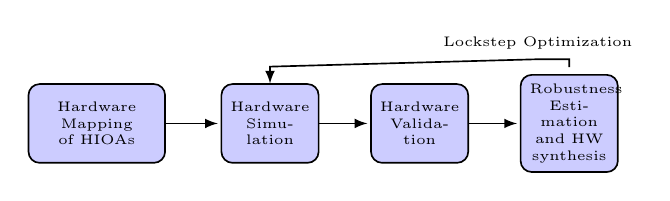
\begin{tikzpicture}[->,>=stealth',shorten >=1pt,auto,semithick,transform shape]
	%\tikzstyle{every state}=[rectangle,rounded corners,minimum height =2.5cm, text width=0.5cm, text centered,fill=purple!20,text=black,line width=0.1mm]
	\tikzstyle{every state} = [draw,rectangle,rounded corners,fill=blue!20,text width=1.5cm,text centered,minimum height=10mm,node distance = 1cm]
	\tikzstyle{block2} = [draw,rectangle,rounded corners,fill=blue!20,text width=1cm,text centered,minimum height=10mm,node distance = 1cm]
	\tikzstyle{block} = [draw,rectangle,rounded corners,fill=blue!20,text width=1cm,text centered,minimum height=10mm,node distance = 1cm]
	\tikzstyle{block1} = [draw,rectangle,rounded corners,fill=blue!20,text width=2.5cm,text centered,minimum height=15mm,node distance = 3cm]
	\tikzstyle{block3} = [draw,rectangle,rounded corners,fill=blue!20,text width=3.8cm,text centered,minimum height=15mm,node distance = 3cm]
	
%	\node[block2] (T1) at (1,1) {FSM specification of Plant and controller HIOAs \\ 
		
%	} ;
	\node[state,font=\tiny] (T2) at (1,3.5) {Hardware Mapping of HIOAs \\  
};
	\node[block2,font=\tiny] (T3) at (3.2,3.5) {Hardware Simulation \\  
};
	
	\node[block2,font=\tiny] (T4) at  (5.1,3.5) {Hardware Validation \\  
};
	%\draw[<-, dashed]([xshift=0cm]T1.west) -- node[above] {Initial} ++(-1cm, 0cm);
	\node[block,font=\tiny] (T5) at  (7,3.5) {Robustness Estimation and HW synthesis \\  
	};
	
	
%	\draw[>=latex,->]  ([xshift= 0pt] T1.north) -- ([xshift= 0pt]T2.south) node [midway,below] { };
	\draw[>=latex,->]  ([xshift= 0pt] T2.east) -- ([xshift= 0pt]T3.west) node [midway,below] { };
	\draw[>=latex,->]  ([xshift= 0pt] T3.east) -- ([xshift= 0pt]T4.west) node [midway,below] { };
	\draw[>=latex,->]  ([xshift= 0pt] T4.east) -- ([xshift= 0pt]T5.west) node [midway,below] { };
	\draw[>=latex,->]  ([xshift= 0pt ,yshift = 2.5pt] T5.north) |- ++(-0.4,0.1) node [right,above,font=\tiny] { Lockstep Optimization } --  ([xshift= 0pt,yshift = 6pt]T3.north) -| ++(0, -0.25)  ;
	
	
	\end{tikzpicture}
	\caption{Hybrid Systems Co-Simulation Flow} \label{fig:}
	
\end{figure}
 \section{Syntax and Semantics of HIOA}
Here we give brief definition of HIOA and then demonstrate it with an example of Human Factor model \citep{Ro2018} based Car following model \citep{bevrani2012evaluation}. This is taken as a running example in this paper. 
The model proposed in \citep{Ro2018} is a compositional framework that incorporates human factors with the car following models (CFM) \citep{bevrani2012evaluation}, the later being our kinematic model. There are different \textit{modes} introduced to model the human factors in the human factor model (HFM), like \textit{Short Delay}, \textit{Long Delay} or \textit{Inattentive}. The kinematic model behaves differently based on these modes.  Each vehicle is a \textit{composition} of HFM and a \textit{kinematic} model. 
 HFM estimates the velocity \grcap{\textit{v\textsubscript{n-1}}} and position \grcap{\textit{x\textsubscript{n-1}}} at time '\textit{t}' on the basis of position and velocity of the leader vehicle .i.e. {\textit{v\textsubscript{n-1}} and \textit{x\textsubscript{n-1}}. And then the estimated relative velocity  and relative spacing are computed by equation 1 and 2, is also shown in figure 3. 	
	
The overall composition is a vehicular cluster as shown in Figure 2, in which each vehicle is running concurrently and we take composition of two vehicles, where in the velocity and position of the leading vehicle is passed to the following vehicle, here, in this case $\textit{v\textsubscript{0}},  $\textit{x\textsubscript{0}} from leader vehicle 0 is passed to the following vehicle 1 and so on.
	\begin{equation}
	\Delta \textit{v}\textsubscript{n}(t) = \grcap{\textit{v}}\textsubscript{n-1}(t) -\textit{v}\textsubscript{n}(t) \label{eq} 
	\end{equation}
	\begin{equation}
	\Delta \textit{x}\textsubscript{n}(t) = \textit{x}\textsubscript{n}(t) - \grcap{\textit{x}}\textsubscript{n-1}(t)  \label{eq}
	\end{equation}
\subsection{Definition Of Hybrid Input Output Automata}
Hybrid Input Output Automata (HIOA) is commonly used for modeling cyber-physical systems \citep{Alur1994}. The overall system process certain Inputs, generates certain outputs and is divided into number of operational states called \textit{locations} which describe discretized continuous process. Here each state captures certain operational dynamics which are specified by a set of ODEs that indicate the rate change of continuous variables. In a given state, the continuous variables evolve  with time over to a certain point which is decided by a set of invariants applicable onto that state. As long as control resides in a particular state, it should conform to the invariant conditions. HIOA model can make state transitions based on the \textit{guard} conditions. Once a given \textit{guard} is satisfied,  a transition from one state to another can take place and any variables associated with the transition can be updated instantaneously.

Definition 1: A hybrid Input Output Automaton (HIOA)\citep{Lygeros1999} is S = \textless\textit{Q},\textit{X},\textit{V},\textit{Y},\textit{Init},\textit{f},\textit{h},\textit{E},\textit{G},\textit{R},\textit{$\delta$}\textgreater where  :
\begin{itemize}
	\setlength{\itemsep}{-12pt}
	\setlength{\parskip}{0pt}
	\item\textit{Q} is a set of discrete locations. \newline
	\item\textit{X} is a finite set of continuous variables. \newline
	\item\textit{I} is finite set of input variables.We assume \textit{I} =  \textit{\(I_{D} \cup I_{C}\)} which is nothing but union of discrete and continuous inputs in their respective domains.\newline
	\item \textit{O} is finite set of output variables and  \textit{O} =  \textit{\(O_{D} \cup O_{C}\), \textit{\(O_{D}\)}} is a finite set of discrete variables while \textit{\(O_{C}\)} is a collection of continuous  variables. \newline
	\item \textit{Init} \(\subseteq \{q_{0}\} \times X \times O\), such that there is exactly one \(q_{0} \in Q\) , is the singleton initial location.\newline
	\item \(f  : Q \times X \times I \to  \mathbb{R}^\norm{X}\)   is a vector field.Function \textit{f(q,x,i)} is globally \textit{Lipschitz} continuous in \textit{x} $\in$ X  and \textit{i} $\in$ I.  \newline
	\item \(h : Q \times X \to O \) is a  vector field. \newline
	\item \(Inv :Q \to {2}^{X \times I}\) assigns to each \(q  \in Q\) is an invariant set. \newline
	\item \(E \subset Q \times Q\) is a collection of discrete edges.\newline
	\item \(G :E \to {2}^{X \times I}\) assign to each  \(e =(q, \dot{q}) \in E \) is a guard. \newline
	\item \(R :E \times X \times I \to {2}^{X \times O} \) assigns to each   \(e =(q, \dot{q}) \in E \) 
	\(x \in X , v \in I \) is a reset relation.\newline
	\item \textdelta  :  It is the duration of any discrete executions step so that the elapsed time at any time step \(k \in \mathbb{N}\) can be computed as 
	\( k \times \delta \) .
\end{itemize}


\begin{figure}
	

	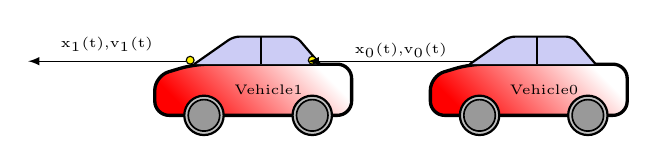
\begin{tikzpicture}

	\tikzset{
	big dot/.style={circle, draw, inner sep=0pt, minimum size=1mm, fill=yellow},
	input/.style={draw, trapezium, trapezium left angle=60, trapezium right angle=120,
		line width=1.2pt, fill={rgb:black,1;white,2}},
	obstacle/.style={draw, trapezium, trapezium left angle=120, trapezium right angle=60,
		line width=1.2pt, fill={rgb:black,1;white,2}},
	flash/.style args={#1:#2}{postaction=decorate,decoration={name=markings,
			mark=at position #1 with {%
				\draw[fill=#2, line width=.75\pgflinewidth, line cap=round, line join=round]
				(+\pgflinewidth,+7\pgflinewidth)   -- ++ ( left:+2\pgflinewidth) 
				-- (+-4\pgflinewidth,+-\pgflinewidth) -- ++ (right:+5\pgflinewidth)
				-- (+-\pgflinewidth,+-7\pgflinewidth) -- ++ (right:+2\pgflinewidth)
				-- (+4\pgflinewidth,\pgflinewidth)    -- ++ (left:+5\pgflinewidth)
				-- cycle;}}}
}


\begin{scope}[scale = 0.5]
\shade[top color=red, bottom color=white, shading angle={135}]
[draw=black,fill=red!20,rounded corners=1.2ex,very thick] (5.5,.5) -- ++(0,1) -- ++(1,0.3) --  ++(3,0) -- ++(1,0) -- ++(0,-1.3) node [midway,font=\tiny,xshift=-30pt] {Vehicle1 } --cycle ;% -- (1.5,.5);% -- cycle;
\draw[very thick, rounded corners=0.5ex,fill=black!20!blue!20!white,thick]  (6.5,1.8) -- ++(1,0.7) -- ++(1.6,0) -- ++(0.6,-0.7);%-- (2.5,1.8) ;
\draw[thick]  (8.2,1.8) -- (8.2,2.5);
\draw[draw=black,fill=gray!50,thick] (6.75,.5) circle (.5);
\draw[draw=black,fill=gray!50,thick] (9.5,.5) circle (.5);
\draw[draw=black,fill=gray!80,semithick] (6.75,.5) circle (.4);
\draw[draw=black,fill=gray!80,semithick] (9.5,.5) circle (.4);
\end{scope}

\node[big dot](T1) at (7,0.95){};
\node[big dot](T2) at (4.75,0.95){};
\node[big dot](T3) at (3.2,0.95){};
\draw[>=latex,->] ([yshift= -0.35pt] T1.east)   -- ([yshift= -0.35pt] T2.west)  node [midway,font=\tiny,yshift=4pt] {x\textsubscript{0}(t),v\textsubscript{0}(t)};  ;

\draw[>= latex,->] ([yshift= -0.35pt] T3.west)   --  node [midway,above,font=\tiny] {x\textsubscript{1}(t),v\textsubscript{1}(t)} ++(-2cm,-0cm);
% {x\textsubscript{1}(t),v\textsubscript{1}(t)};  ;
%\draw[>=latex,<-]  ([yshift= 3pt] au.east) --  node [midway,above,font=\tiny] {v\_org} ++(2cm,-0cm);

\begin{scope}[scale = 0.5]
\shade[top color=red, bottom color=white, shading angle={135}]
[draw=black,fill=red!20,rounded corners=1.2ex,very thick] (12.5,.5) -- ++(0,1) -- ++(1,0.3) --  ++(3,0) -- ++(1,0) -- ++(0,-1.3) node [midway,font=\tiny,xshift=-30pt] {Vehicle0 } --  cycle;
\draw[very thick, rounded corners=0.5ex,fill=black!20!blue!20!white,thick]  (13.5,1.8) -- ++(1,0.7) -- ++(1.6,0) -- ++(0.6,-0.7);% -- (2.5,1.8);%top
\draw[thick]  (15.2,1.8) -- (15.2,2.5);
\draw[draw=black,fill=gray!50,thick] (13.75,.5) circle (.5);
\draw[draw=black,fill=gray!50,thick] (16.5,.5) circle (.5);
\draw[draw=black,fill=gray!80,semithick] (13.75,.5) circle (.4);
\draw[draw=black,fill=gray!80,semithick] (16.5,.5) circle (.4);
\end{scope}
	
\end{tikzpicture}
\caption{Vehicle Composition} \label{fig:}
\end{figure}
\begin{figure}
	%[every node/.style={minimum height={1.5cm},thick,align=center}]
	\tikzstyle{decision} =[diamond,draw,fill=blue!50]
	\tikzstyle{line} = [draw,-latex']
	\tikzstyle{elli} = [draw,circle,fill=none,node distance = 2.2cm]
	\tikzstyle{block} = [draw,rectangle,rounded corners,fill=blue!50,text width=1.2cm,text centered,minimum height=5mm,node distance = 0.5cm]
	\tikzstyle{block1} = [draw,rectangle,rounded corners,fill=blue!50,text width=1.5cm,text centered,minimum height=5mm,node distance = 2.7cm]
	\begin{tikzpicture}
	
	\node[block,font=\tiny](hfm) {Human Factor Model};
	\node[elli,right of=hfm,font=\tiny](minus) {Minus};
	\node[block1,right of=minus,font=\tiny](cfm) {Car Follower Model};
	\draw[<-, solid](hfm.180) -- node[above,font=\tiny] {v\textsubscript{n-1}(t) } ++(-1cm,-0cm);
	\draw[<-, solid](hfm.180) -- node[below,font=\tiny] {x\textsubscript{n-1}(t) } ++(-1cm,-0cm);
	
	
	\path [line] (hfm) -- node[yshift=0.2cm,font=\tiny] {\grcap{v\textsubscript{n-1}(t)}} (minus);%{V};%\textsuperscript{^}\textsubscript{n-1}};
	\path [line] (hfm) -- node[yshift=-0.2cm,font=\tiny] {\grcap{x\textsubscript{n-1}(t)}} (minus);%{V};%\textsuperscript{^}\textsubscript{n-1}};
	\path [line] (minus) -- node[yshift=0.2cm,font=\tiny] {$\Delta$\grcap{x\textsubscript{n}(t)}} (cfm);
	\path [line] (minus) -- node[yshift=-0.2cm,font=\tiny] {$\Delta$\grcap{v\textsubscript{n}(t)}} (cfm);
	\draw[->]  (cfm) -- node {} ++(0,0.9cm) -| (minus) node[above,pos=0.25,font=\tiny] {\textit{v}\textsubscript{n}(t),\textit{x}\textsubscript{n}(t)} node[pos=0.85] {};
	%\draw[->, solid](cfm.0) -- node[right] {v\textsubscript{n-1}(t+ \textdelta) , x\textsubscript{n-1}(t+\textdelta) } ++(-0.4cm,0cm);
	\draw[->, solid](cfm.0) -- node[above,font=\tiny] {v\textsubscript{n-1}(t+ \textdelta) } ++(1.3cm,-0cm);
	\draw[->, solid](cfm.0) -- node[below,font=\tiny] {x\textsubscript{n-1}(t+ \textdelta) } ++(1.3cm,-0cm);
	
	
	\end{tikzpicture}
	\caption{Human factor and kinematics model composition} \label{fig1}
\end{figure}
\subsubsection{Human Factor Model as an HIOA}
 Figure 4 shows the HIOA of Human Factor Model(HFM) \citep{Ro2018}. The HFM estimates kinematics of the leading vehicle in a Human Factor Based Car following model paradigm. The HFM consists of four states/locations  illustrating  \textit{normal} and \textit{distracted} driving scenarios. These are \textit{Attentive} (Represents normal driving),\textit{short delay} (represents normal reaction delay to an event),\textit{Inattentive} (Inattentive driving situation) and \textit{long delay} (Longer reaction time due to distraction).
 The variables which constitute the HIOA ingredients are defined as follows:

\hspace*{1cm} $\bullet$ \textit{X} = \{\textit{t},\grcap{\textit{v\textsubscript{n-1}}},\grcap{\textit{a\textsubscript{n-1}}},\grcap{\textit{x\textsubscript{n-1}}}, $\textit{v}_{n-1}^{pre}$ \} , with X = $\real$ \\
\hspace*{1.4cm} $\bullet$ \textit{I} = \textit{I\textsubscript{C}} = \{ \textit{v}\textsubscript{n-1},\textit{x}\textsubscript{n-1} \}, with  $\boldsymbol{I}$ = $\real^{2}$ \\
 \hspace*{1.4cm} $\bullet$\textit{O} = \textit{O\textsubscript{C}} = \{$\grcap{\textit{v}}_{n-1}^{out }$, $\grcap{\textit{x}}_{n-1}^{out }$\}, with O = $\real$ 


Here \textit{X} is the finite collection of state variables, while \textit{I} is the set of input variables, \textit{t} is the time,$\grcap{\textit{a}\textsubscript{n-1}}$ is the estimated leader acceleration and {${\textit{v}_{n-1}^{pre}}$} is a variable that temporarily stores the value of {${\textit{v}_{n-1}}$} internally. Here the Output variables are responsible for sending out the estimated values of velocity and acceleration.
The vector field \textit{f} in the Equation 3 defines basic ODE and since kinematics (e.g. \textit{\grdot{\grcap{v\textsubscript{n-1}}}} = \textit{\grcap{a\textsubscript{n-1}}}) are to be the same so \textit{f} is to be identical in all locations. Here \textit{\grdot{t}} represents the time flow.The output variables are updated by the function \textit{h} given by Equation 4. It should be noted that the most recent value of output variables is tracked by this equation. The invariants \textit{(Inv)} are the conditions for \textit{self loop} in each location are displayed in the location box. For example, t $\le$ 1.9 is invariant for \textit{short delay} state. Finally, the guards and output variables are shown as labels over the transition arrows and are displayed in Table I. The HIOA for this model is displayed in Figure 4.
\begin{gather}
	\textit{f}(\textit{t},\textit{\grcap{a\textsubscript{n-1}},\grcap{v\textsubscript{n-1}},\grcap{x\textsubscript{n-1}}}) =\begin{bmatrix} \grdot{\grcap{\textit{v\textsubscript{n-1}}}} \\
	\grdot{\grcap{\textit{x\textsubscript{n-1}}} \\       \grdot{\textit{t}}} 
	\end{bmatrix} = 
	\begin{bmatrix} \grcap{\textit{a\textsubscript{n-1}}} \\
	\grcap{\textit{v\textsubscript{n-1}} \\ 1} 
	\end{bmatrix}
\end{gather}

\begin{align}
\textit{h}(\grcap{v\textsubscript{n-1}},\grcap{x\textsubscript{n-1}}) =\begin{bmatrix} \grcap{\textit{v}}_{n-1}^{out} \\
\grcap{\textit{x}}_{n-1}^{out} \\ 
\end{bmatrix} = 
\begin{bmatrix} \grcap{\textit{v\textsubscript{n-1}}} \\
\grcap{\textit{x\textsubscript{n-1}}} \\ 
\end{bmatrix}
%\textit{dx} = \textit{v} \textit{dt}\\
%\textit{dv} = \textit{a} \textit{dt}
\end{align}
When the control is in \textit{attentive} state, estimated velocity and position of the leader are computed along with actual parameters. When the control logic moves from \textit{attentive} to \textit{short delay}, the estimated position and velocity are saved and the start of the reaction time is flagged. Hence $\textit{v}_{n-1}^{pre}$ = $\textit{v}\textsubscript{n-1}$,$\grcap{\textit{X}}_{n-1}$ = ${\textit{X}_{n-1}}$.
And when the control logic moves back to the \textit{attentive} state, estimated values of acceleration are computed as $\grcap{\textit{a}\textsubscript{n-1}}$ =($\textit{v}\textsubscript{n-1}$ -  $\textit{v}_{n-1}^{pre}$)/t. %$\frac{$\textit{v_{n-1}}$}{b}$%\frac{$\textit{v}\textsubscript{n-1}$ -  $\textit{v}_{n-1}^{pre}$}{t}

In a similar way, the estimated acceleration is computed when the control logic moves from \textit{long delay} to \textit{attentive} mode.
It should be noted that entering the delay locations represents the beginning of reaction delay,  while, on the other hand exiting the delay locations represents end of the reaction delay. Each guard is a boolean condition which enables transition on being true. During each transition the corresponding reset function is executed to assign new values to the local variables which is listed in Table I. The common set of variable updates performed while staying in any of the locations in HIOA of Figure 4 are :
 $\grdot{\grcap{\textit{v}}}_{n-1}$ = $\grcap{\textit{a}}_{n-1}$ , $\grdot{\grcap{\textit{x}}}_{n-1}$ = $\grcap{\textit{v}}_{n-1}$,\grdot{t} = 1,  $\grcap{\textit{v}}_{n-1}^{out}$ =$\grcap{\textit{v}}_{n-1}$,$\grcap{\textit{x}}_{n-1}^{out}$ =$\grcap{\textit{x}}_{n-1}$.\\
 \begin{figure}
	
	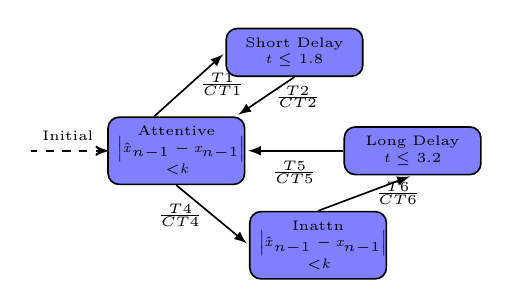
\begin{tikzpicture}[->,>=stealth',shorten >=1pt,auto,semithick,transform shape]
	%\tikzstyle{every state}=[rectangle,rounded corners,minimum height =1.2cm, text width=1.2cm, text centered,fill=purple!20,text=black,line width=0.3mm]
	\tikzstyle{every state} = [draw,rectangle,rounded corners,fill=blue!50,text width=1.5cm,text centered, minimum height=2mm,node distance = 1cm]
	
	\node[state,font=\tiny] (T1) at (1,1) {Attentive \\ 
	$\abs{\grcap{\textit{x}}_{n-1} - \textit{x}_{n-1}}$ \textless $\textit{k}$
   };

	\node[state,font=\tiny] (T2) at (2.5,2.25) {Short Delay \\  
		$\textit{t}$ $\le$ 1.8};
	\node[state,font=\tiny] (T3) at (4,1) {Long Delay\\  
		$\textit{t}$ $\le$ 3.2};
	
	\node[state,font=\tiny] (T4) at  (2.8,-0.2) {Inattn \\  
		$\abs{\grcap{\textit{x}}_{n-1} - \textit{x}_{n-1}}$ \textless $\textit{k}$};
	\draw[<-, dashed]([xshift=0cm]T1.west) -- node[above,font=\tiny] {Initial} ++(-1cm, 0cm);

	
	\draw[>=latex,->]  ([xshift= 0pt] T3.west) -- ([xshift= 0pt]T1.east) node [midway,below,font=\tiny] {$\frac{T5}{CT5}$ };
	\draw[>=latex,->]  ([xshift= -8pt] T1.north) -- ([xshift= 0pt]T2.west) node [midway,right,font=\tiny] {$\frac{T1}{CT1}$};	
	\draw[>=latex,->]  ([xshift= 0pt] T2.south) -- ([xshift= 0pt]T1.30) node [midway,right,font=\tiny] {$\frac{T2}{CT2}$ };
	
	
	\draw[>=latex,->]  ([xshift= 0pt] T4.north) -- ([xshift= 0pt]T3.south) node [midway,right,font=\tiny] {$\frac{T6 }{CT6}$};
	;	
	
	\draw[>=latex,->]  ([xshift= 0pt] T1.south) -- ([xshift= 0pt]T4.west) node [midway,left,font=\tiny] {$\frac{T4 }{CT4}$};
	
	\end{tikzpicture}
	\caption{Human Factor Model HIOA.Table II details the Transition labels.} \label{fig:}
\end{figure}
\subsubsection{Kinematics Model}
Kinematics model is the Car Follower model \citep{bevrani2012evaluation} which computes the follower's motion parameters using the equation 5.
\begin{equation}
a\textsubscript{n}(t) = v\textsubscript{n}(t)\frac{\Delta v\textsubscript{n}(t)}{\Delta x\textsubscript{n}(t)}\label{eq}
\end{equation}
where 
\textit{a\textsubscript{n}(t)} = Acceleration of the vehicle \textit{n} at time t, \textit{v} is speed of the follower vehicle, \textit{\textDelta x\textsubscript{n}(t)} is relative spacing between the follower and the leader vehicle.
\textit{\textDelta v\textsubscript{n}(t)} is relative velocity between the follower and leader vehicle.

These differences are fed to the equation 3 above and finally the car follower's acceleration is computed. 
As depicted in Figure 3 the compositional framework incorporates human factors\citep{Ro2018} with the kinematic model\citep{bevrani2012evaluation} which has a single state and at every new iteration new follower values are calculated.
\section{Hardware modeling of Cyber Physical Systems}
\subsection{Overview}
The generic hardware model consists of a Plant and a Controller Unit which models their respective FSMs. Description of each module is given as follows: (1) Plant: It has it's respective FSM(s) coded for realizing the functionality. They interact with the Arithmetic unit for doing IEEE 754 SP computations. (2) The Arithmetic unit has various tasks implemented for doing floating point computations. (3) Controller functionality is realized by a control unit which controls the plant activity and FSM(s) associated.  
(4) Different properties (MITL, Parameteric and LTL ) are implemented which verify the controller correctness. These properties constitute the Verification Engine. (6) The clock generator provides the clock frequency on which the design will work and all FSM(s) will operate. All these are represented in Figure 5.
\begin{table}[]
	\centering
	\caption{Variable Update legend on state Transition}
	\label{my-label}
	\scalebox{0.60}{%
		\begin{tabular}{ |c|c| }
			\hline \hline
			\multicolumn{2}{|c|}{Leader kinematics update} \\ \hline
			\multicolumn{2}{|c|}{Guards for Human Factor Model}\\ \hline
			Label & Values \\ \hline
			T1 & $\abs{\grcap{\textit{x}}_{n-1} - \textit{x}_{n-1}}$ $\geq$ $\textit{k}$ \\
			T2 & ${\text{t}\geq 0.5}$\\
			T4 & $\abs{\grcap{\textit{x}}_{n-1} - \textit{x}_{n-1}}$ $\geq$ $\textit{k}$ \& \textit{t} $\geq$ 8 \\
			T5 & ${\grcap{\textit{v}}_{n-1}^{'}= \textit{v}_{n-1}}$ ,
			${\grcap{\textit{a}}_{n-1} = \frac{\textit{v}_{n-1} -\textit{v}_{n-1}^{pre} }{\text{t}}}$ \\
			T6 &  ${\text{t}\geq 0.5}$\\
			Initial & \textit{v}\textsubscript{n} = 0.002, \textit{x}\textsubscript{n}= 0.1, $\Delta$\textit{v}\textsubscript{n}=5.75,$\Delta$\textit{x}\textsubscript{n}=0.1 , K = 0.845 \\ \hline
			\multicolumn{2}{|c|}{Variable Update on state Transition}\\ \hline
			\hline
			Label & Values \\ \hline
			
			CT1 & \textit{t'}=0 ,${\grcap{\textit{x}}_{n-1}^{`}= \textit{x}_{n-1}}$,
			${\textit{v}_{n-1}^{{pre}{'}}= \textit{v}_{n-1}}$ \\
			CT2 & \textit{t'}=0, ${\grcap{\textit{v}}_{n-1}^{'}= \textit{v}_{n-1}}$ ,
			${\grcap{\textit{a}}_{n-1} = \frac{\textit{v}_{n-1} -\textit{v}_{n-1}^{pre} }{\text{t}}}$ \\
			CT4 & $\phi$ \\
			CT5 & \textit{t'}=0, ${\grcap{\textit{v}}_{n-1}^{'}= \textit{v}_{n-1}}$ ,
			${\grcap{\textit{a}}_{n-1} = \frac{\textit{v}_{n-1} -\textit{v}_{n-1}^{pre} }{\text{t}}}$ \\
			CT6 & \textit{t'}=0, ${\grcap{\textit{x}}_{n-1}^{`}= \textit{x}_{n-1}}$,
			${\textit{v}_{n-1}^{{pre}{'}}= \textit{v}_{n-1}}$ \\
			
			
			
			\hline
			
	\end{tabular}}
\end{table}

 
\subsection{Mapping HIOA to Hardware}
Every HIOA is mapped as a finite state machine (FSM) in hardware.
Various constituents of the HIOA are extracted like invariants, input, output variables and guard statements. They are mapped as per FSM coding rules. The rules in brief are as follows:
(1) The number of locations/states in the translated FSM are same as HIOA. (2) The \textit{lockstep} value of HIOA is taken as the clock period of the FSM
(3) Each intra-state transition is translated into a state loop, evolving the continuous variables in the state, until the invariant condition holds. For example, in figure 4, \textit{|} \grcap{\textit{x\textsubscript{n-1}}}  - \textit{x\textsubscript{n-1}}\textit{|} < \textit{k} is the invariant condition self loop condition in \textit{attentive} state. (4) Each ODE is solved analytically at every state and every guard condition serves the same role .i.e these are rules for state transition. (5) If there is a network of FSMs, all FSMs are synced by the clock period we choose, which is also used for iterating the FSM states. The FSM for Human factor model is presented in Figure 6. 
Every ODE is translated into a difference equation using the Euler approximation technique \citep{bulirsch1966numerical}. We present the Human factor model FSM based on it's HIOA  in Figure 6.
The interface signals for our running example are shown in Figure 7. The HFM FSM and it's associated Arithmetic unit defines the controller, while the kinematic FSM with it's arithmetic unit realize the Plant. System verilog assertions with IEEE754 to real converter block defines the Verification engine. The converter block converts the Single precision values into floating point  for better observability. As indicated, the human factor model outputs estimated(x\_est,v\_est,a\_est) and original(x\_org,v\_org,a\_org) motion values(x=location, v=velocity, a=acceleration) of the leader vehicle. These are used by the kinematic model to compute it's motion parameters at next iteration. The clock generator module generates the clock which is passed to all the modules. Upon synthesis, the PLL module replaces this generator for real time clock realization.
\subsection{Robust Execution of HIOA}
To ensure that the hardware works as per the functionality various MITL properties are defined. To check if the properties are robust we rely on off line robustness estimation \textit{H($\phi$)} procedure and assumptions, defined in \citep{fainekos2007robust}. By Robustness estimate we mean to define the robustness of the specifications with respect to the timing constraints. In other words, discrete time signal must robustly satisfy all the MITL specifications with respect to a clock  used in simulation $\Delta$$\tau$. Based on this clock we compute the robustness estimate. Now, if \textit{H($\phi$)} $\geq$ $\Delta$$\tau$ x $\epsilon$ , then the $\Delta$$\tau$ is optimum clock which will cover all the events in simulation. Here $\epsilon$ is the \textit{Lipschitz constant} of the equation under consideration. For instance, the first property for our running example in Table V is valid for $\Delta$$\tau$ = 0.08 , as \textit{H($\phi$)} = 8.56 ,\textit{$\epsilon$ x $\Delta$$\tau$} = 7.72, hence, \textit{H($\phi$)} $\geq$ $\Delta$$\tau$ x  $\epsilon$  holds , while on the contrary if we chose $\Delta$$\tau$ = 0.192, the equation does not hold true, because \textit{H($\phi$)} < $\Delta$$\tau$ x $\epsilon$. Consequently, for this $\Delta$$\tau$, various simulation events will be missed  where the property has to justify the hardware correctness.

\begin{figure}
	
	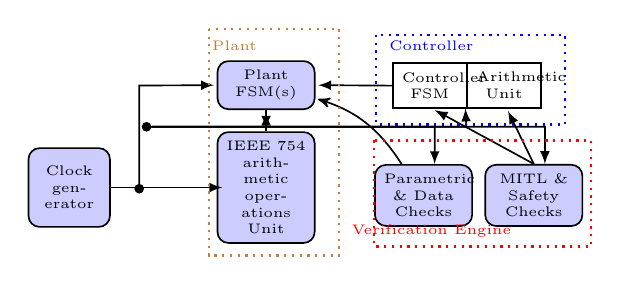
\begin{tikzpicture}[->,>=stealth',shorten >=1pt,auto,semithick,transform shape]
	%\tikzstyle{every state}=[rectangle,rounded corners,minimum height =2.5cm, text width=0.5cm, text centered,fill=purple!20,text=black,line width=0.1mm]
	\tikzstyle{every state} = [draw,rectangle,rounded corners,fill=blue!20,text width=2cm,text centered,minimum height=20mm,node distance = 1cm]
	\tikzstyle{block2} = [draw,rectangle,rounded corners,fill=blue!20,text width=1.0cm,text centered,minimum height=5mm,node distance = 1cm]
	\tikzstyle{block} = [draw,rectangle,rounded corners,fill=blue!20,text width=2.0cm,text centered,minimum height=15mm,node distance = 3cm]
	\tikzstyle{block1} = [draw,rectangle,rounded corners,fill=blue!20,text width=1.0cm,text centered,minimum height=15mm,node distance = 3cm]
	\tikzstyle{block3} = [draw,rectangle,rounded corners,fill=blue!20,text width=0.8cm,text centered,minimum height=10mm,node distance = 1cm]
	\tikzstyle{block4} = [draw,rectangle,rounded corners,fill=blue!20,text width=1cm,text centered,minimum height=5mm,node distance = 1cm]
	\tikzset{
		big dot/.style={circle, draw, inner sep=0pt, minimum size=1mm, fill=black},
		input/.style={draw, trapezium, trapezium left angle=60, trapezium right angle=120,
			line width=1.2pt, fill={rgb:black,1;white,2}},
		obstacle/.style={draw, trapezium, trapezium left angle=120, trapezium right angle=60,
			line width=1.2pt, fill={rgb:black,1;white,2}},
		flash/.style args={#1:#2}{postaction=decorate,decoration={name=markings,
				mark=at position #1 with {%
					\draw[fill=#2, line width=.75\pgflinewidth, line cap=round, line join=round]
					(+\pgflinewidth,+7\pgflinewidth)   -- ++ ( left:+2\pgflinewidth) 
					-- (+-4\pgflinewidth,+-\pgflinewidth) -- ++ (right:+5\pgflinewidth)
					-- (+-\pgflinewidth,+-7\pgflinewidth) -- ++ (right:+2\pgflinewidth)
					-- (+4\pgflinewidth,\pgflinewidth)    -- ++ (left:+5\pgflinewidth)
					-- cycle;}}}
				}
	
	\node[block3,,font=\tiny] (T2) at (2.9,4.2) {Clock generator \\  
	};
	\node[block2,font=\tiny] (T3) at (5.4,5.5) { Plant FSM(s) \\  
	};
	\node[block2,font=\tiny] (T10) at (5.4,4.2) { IEEE 754 arithmetic operations Unit\\  
	};
	\path (T2) (T2.east)++(0,0) |- ++(-0.8,-1.1) -- node[big dot] (bigdot1) {} (T3);
	
	\path (T2) (T2.east)++(0,0) |- ++(-0.35,0.4) -- node[big dot] (bigdot2) {} (T3);
	\draw[>=latex,->] ([yshift= 0pt] bigdot1.north) |-  ++(0cm,1.25cm)   -- (T3.west) {}  ;
	
	\node[draw,anchor=south west,text width = 7mm,text centered,minimum width=5mm,minimum height=5mm,,font=\tiny] (T4) at (7,5.2) {Controller FSM   };
	\node[draw,anchor=north east,text width=7mm,text centered,minimum height=5mm,font=\tiny] (T5) at (8.9,5.79) { Arithmetic Unit};
	%\node[block1] (T4) at  (7.5,5.5) {Snoop FSM \\  	};
	%\node[block4] (T5) at  (7.5,4.5) {Control Unit \\  	};
	%\draw[<-, dashed]([xshift=0cm]T1.west) -- node[above] {Initial} ++(-1cm, 0cm);
	\node[block4,,font=\tiny] (T6) at  (8.8,4.1) {MITL \& Safety Checks \\  	};
	%\node[block4] (T7) at  (9.5,3.5) {Safety checks \\	};
	\node[block4,font=\tiny] (T8) at  (7.4,4.1) {Parametric \& Data Checks \\ };
	%\node[block4] (T9) at  (7.1,3.5) {Trivial Propeties \\ 	};
	%	\node[block4] (T10) at  (7.1,3.5) {Control Unit \\  
	%	};
	\draw[>=latex,->] ([yshift= 0pt] bigdot2.east) -|  ++(4cm,0cm)   -- ([xshift=-14.0pt,yshift = 1pt]T5.south) {}  ;
	\draw[>=latex,->] ([yshift= 0pt] bigdot2.east) -|  ++(3.6cm,0cm)   -- ([xshift=4.0pt,yshift = -1pt]T8.north) {}  ;
	\draw[>=latex,->] ([yshift= 0pt] bigdot2.east) -|  ++(5cm,0cm)   -- ([xshift=4.0pt,yshift = -1pt]T6.north) {}  ;
	
	
	
	\draw[>=latex,->]  ([xshift= 0pt] T2.east) -- ([xshift= 3pt]T10.west) node [midway,below] { };
	%\draw[>=latex,->]  ([xshift= 0pt] T2.east) -- ([xshift= 0pt]T3.west) node [midway,below] { };
	%	\draw[>=latex,->]  ([xshift= 0pt] T5.east) -- ([xshift= 0pt]T4.west) node [midway,below] { };
	\draw[>=latex,->]  ([xshift= 0pt] T4.west) -- ([xshift= 0pt]T3.east) node [midway,below] { };
	\draw[>=latex,->]  ([xshift= 0pt] T6.north) -- ([xshift= 1pt]T4.south) node [midway,below] { };
	\draw[>=latex,->]  ([xshift= 0pt] T6.north) -- ([xshift= 1pt]T5.south) node [midway,below] { };
	\draw[>=latex,->]  ([xshift= 0pt] T3.south) -- ([xshift= 0pt]T10.north) node [midway,below] { };
	\draw[>=latex,->]  ([xshift= 0pt] T10.north) -- ([xshift= 0pt]T3.south) node [midway,below] { };
	\path[->]          (T8)  edge   [bend right=20]   node {} (T3);
	\draw[red,thick,dotted] ($(T8.north west)+(0,0.30)$) node[font=\tiny] at (7.5,3.65){Verification Engine} rectangle ($(T6.south east)+(0.1,-0.25)$)  ;
	\draw[blue,thick,dotted]     ($(T4.north west)+(-0.2,0.35)$) node[font=\tiny] at(7.5,6){Controller}rectangle ($(T5.south east)+(0.3,-0.2)$);
	\draw[brown,thick,dotted]     ($(T3.north west)+(-0.1,0.4)$) node[font=\tiny] at(5,6){Plant}rectangle ($(T10.south east)+(0.3,-0.15)$);
	\end{tikzpicture}
	\caption{Hardware Implementation Overview} \label{fig:}
\end{figure}
\begin{figure}
	
	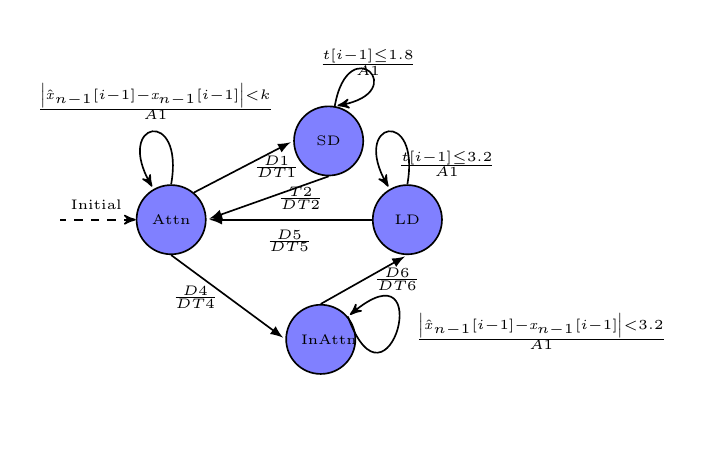
\begin{tikzpicture}[->,>=stealth',shorten >=1pt,auto,semithick,transform shape]
	%\tikzstyle{every state}=[rectangle,rounded corners,minimum height =1.2cm, text width=1.2cm, text centered,fill=purple!20,text=black,line width=0.3mm]
	\tikzstyle{every state} = [circle,fill=blue!50,text width=0.5cm, align=center,text centered,minimum height=0.5mm,node distance = 0.1cm]
	
	
	\node[state,font=\tiny] (T1) at (1,1) {Attn } ;
	\node[state,font=\tiny] (T2) at (3,2) {SD };
	\node[state,font=\tiny] (T3) at (4,1) {LD};
	
	\node[state,font=\tiny] (T4) at  (2.9,-0.52) {InAttn };
	%T1-self loop	
	\draw (T1.90) to[out=80,in=120, distance=1cm] (T1.120);
	\draw (T1)  node[yshift=1.5cm, xshift=-0.2cm,font=\tiny]
	{ {$\frac{\abs{\grcap{\textit{x}}_{n-1}[i-1] - \textit{x}_{n-1}[i-1]} \textless k}
			{A1}$}};
	\draw[<-, dashed]([xshift=0cm]T1.west) -- node[above,font=\tiny] {Initial} ++(-1cm, 0cm);
	
	%T2 self loop
	\draw (T2.80) to[out=80,in=10, distance=1cm] (T2.80);
	\draw (T2)  node[yshift=1cm, xshift=0.5cm,font=\tiny] { {$\frac{t[i-1] \le 1.8}
			{A1}$}};
	%T3 self Loop
	\draw (T3.90) to[out=80,in=120, distance=1cm] (T3.120);
	\draw (T3)  node[yshift=0.71cm, xshift=0.5cm,font=\tiny]
	{ {$\frac{t[i-1] \le 3.2}
			{A1}$}};
%	{ $\textit{t}$ $\le$ 3.2};
	%T4 self Loop
	\draw (T4.40) to[out=-70,in=40, distance=1.5cm] (T4.40);
	\draw (T4)  node[yshift=0.1cm, xshift=2.8cm,font=\tiny]{$\frac{\abs{\grcap{\textit{x}}_{n-1}[i-1] - \textit{x}_{n-1}[i-1]} \textless 3.2}
		{A1}$};
	
%	{ \frac{$\abs{\grcap{\textit{x}}_{n-1}[i-1] - \textit{x}_{n-1}[i-1]}$ \textless $\textit{k}$}{den}};
	
	\draw[>=latex,->]  ([xshift= 0pt] T3.west) -- ([xshift= 0pt]T1.east) node [midway,below,font=\tiny] {$\frac{D5}{DT5}$ };
	\draw[>=latex,->]  ([xshift= 0pt] T1.50) -- ([xshift= 0pt]T2.180) node [midway,right,font=\tiny] {$\frac{D1}{DT1}$};	
	\draw[>=latex,->]  ([xshift= 0pt] T2.270) -- ([xshift= 0pt]T1.0) node [midway,right,font=\tiny] {$\frac{T2}{DT2}$ };
	
	
	\draw[>=latex,->]  ([xshift= 0pt] T4.north) -- ([xshift= 0pt]T3.south) node [midway,right,font=\tiny] {$\frac{D6 }{DT6}$};
	;	
	
	\draw[>=latex,->]  ([xshift= 0pt] T1.south) -- ([xshift= 0pt]T4.west) node [midway,left,font=\tiny] {$\frac{D4 }{DT4}$};
	
	\end{tikzpicture}
	\caption{Human Factor Model HIOA FSM. Table I details Transition labels.} \label{fig:}
\end{figure}
\begin{table}[]
	\centering
	\caption{Variable Update legend on state Transition}
	\label{my-label}
	\scalebox{0.60}{%
	\begin{tabular}{ |c|c| }
		\hline \hline
		\multicolumn{2}{|c|}{Leader kinematics update} \\ \hline
		\multicolumn{2}{|c|}{Guards for Human Factor Model}\\ \hline
		Label & Values \\ \hline
		D1 & $\abs{\grcap{\text{x[i-1]}}_{n-1} - \text{x[i-1]}_{n-1}}$ $\geq$ $\text{k}$ \\
		D2 & ${\text{t[i-1]}\geq 0.5}$\\
		D4 & $\abs{\grcap{\text{x[i-1]}}_{n-1} - \text{x[i-1]}_{n-1}}$ $\geq$ $\text{k}$ \& \text{t[i-1]} $\geq$ 8 \\
		D5 & ${\grcap{\text{v[i-1]}}_{n-1}^{'}== \text{v[i-1]}_{n-1}}$ ,
		${\grcap{\text{a[i]}}_{n-1} == \frac{\text{v[i-1]}_{n-1}[i-1] -\text{v[i-1]}_{n-1}^{pre}}{\text{t[i-1]}}}$ \\
		D6 &  ${\text{t[i-1]}\geq 0.5}$\\
		Initial & \textit{v}\textsubscript{n} = 0.002, \textit{x}\textsubscript{n}= 0.1, $\Delta$\textit{v}\textsubscript{n}=5.75,$\Delta$\textit{x}\textsubscript{n}=0.1 , K = 0.845 \\ \hline
		\multicolumn{2}{|c|}{Variable Update on state Transition}\\ \hline
		\hline
		Label & Values \\ \hline
		
		DT1 & \text{t'}[i]=0 ,${\grcap{\text{x[i]}}_{n-1}^{`}= \text{x[i-1]}_{n-1}}$,
				${\text{v[i]}_{n-1}^{{pre}{'}}= \text{v[i-1]}_{n-1}}$ \\
		DT2 & \grdash{t[i]}=0, ${\grcap{\text{v[i]}}_{n-1}^{'}= \text{v[i-1]}_{n-1}^{`}}$ ,
				${\grcap{\text{a[i]}}_{n-1} = \frac{\text{v[i-1]}_{n-1} -\text{v[i-1]}_{n-1}^{pre} }{\text{t[i]}}}$ \\
		DT4 & $\phi$ \\
		DT5 & \grdash{\text{t[i]}}=0, ${\grcap{\text{v[i]}}_{n-1}^{'}= \text{v[i-1]}_{n-1}}$ ,
		${\grcap{\text{a[i]}}_{n-1} = \frac{\text{v[i-1]}_{n-1} -\text{v[i-1]}_{n-1}^{pre} }{\text{t[i-1]}}}$ \\
		DT6 & \text{t[i]'}=0, ${\grcap{\text{x[i]}}_{n-1}^{`}= \text{x[i-1]}_{n-1}}$,
		${\text{v[i]}_{n-1}^{{pre}{'}}= \text{v[i-1]}_{n-1}}$ \\
		A1 &\text{x[i]}\textsubscript{n-1} = \text{x[i-1]}\textsubscript{n-1} + \text{v[i-1]}\textsubscript{n-1} * $\delta$, \\ &
			\text{v[i]}\textsubscript{n-1} = \text{v[i-1]}\textsubscript{n-1} + \text{a[i-1]}\textsubscript{n-1} * $\delta$,\\ &
			%\text{a[i]}\textsubscript{n-1} = \text{a[i-1]}\textsubscript{n-1} + \text{a[i-1]}\textsubscript{n-1} * $\delta$,\hline
			
			\grcap{\text{x[i]}\textsubscript{n-1}} = \grcap{\text{x[i-1]}\textsubscript{n-1}} + \grcap{\text{v[i-1]}\textsubscript{n-1}} * $\delta$,\\ &
			\grcap{\text{v[i]}\textsubscript{n-1}} = \grcap{\text{v[i-1]}\textsubscript{n-1}} + \grcap{\text{a[i-1]}\textsubscript{n-1}} * $\delta$,\\
			%\grcap{\text{a[i]}\textsubscript{n-1}} = \grcap{\text{a[i-1]}\textsubscript{n-1}} + \text{a[i-1]}\textsubscript{n-1} * $\delta$,
			
			
		
		
	
		\hline
	
	\end{tabular}}
\end{table}
\begin{table}[]
	\centering
	\caption{ Properties for Kinematic Model  }
	\label{my-label}
	\scalebox{0.60}{%
	\begin{tabular}{ |p{0.4cm}|p{7cm}| }
		\hline \hline
		\multicolumn{2}{|c|}{Properties for Car Follower} \\
		\hline
		S.No. & \hspace*{2.7cm} Property \\ \hline
		1 & The Follower velocity should increase if distance from the leader increases\\
		2 & The Follower acceleration should increase if the relative leader velocity increases \\
		3 & The separation between follower and leader should be \textgreater \textit{L}. L is the vehicle size. \\ 
		4 & The Follower's velocity should not be negative. \\
		\hline
		
	\end{tabular}}
\end{table}
\begin{figure}
		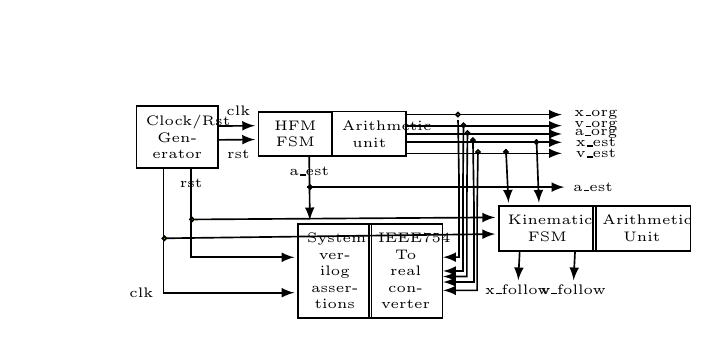
\begin{tikzpicture}[->,>=stealth',shorten >=1pt,auto,semithick,transform shape]
		%\tikzstyle{every state}=[rectangle,rounded corners,minimum height =2.5cm, text width=0.5cm, text centered,fill=purple!20,text=black,line width=0.1mm]
		\tikzstyle{every state} = [draw,rectangle,rounded corners,fill=blue!20,text width=2cm,text centered,minimum height=20mm,node distance = 1cm]
		\tikzstyle{block2} = [draw,rectangle,fill=none,text width=2.7cm,text centered,minimum height=0.5cm,node distance = 2mm]
		\tikzstyle{block} = [draw,rectangle,fill=none,text width=0.7cm,text centered,minimum height=5mm,node distance = 3cm]
		\tikzstyle{block1} = [draw,rectangle,fill=none,text width=0.8cm,text centered,minimum height=7mm,node distance = 3cm]
		
		\tikzstyle{block4} = [draw,rectangle,fill=none,text width=1cm,text centered,node distance = 1cm]
		\tikzstyle{wrapper1} = [draw,rectangle,fill=none,text width=1.0cm,text centered,minimum height=12mm,node distance = 1cm]
		\tikzstyle{block3} = [draw,rectangle,fill=none,text width=0.7cm,text centered,minimum height=3mm,node distance = 3cm]
		%\tikzstyle{block4} = [draw,rectangle,rounded corners,fill=blue!20,text width=1.4cm,text centered,minimum height=10mm,node distance = 1cm]
		\tikzset{
			myarrow/.style={->, >=latex', shorten >=1pt, thick},
			mylabel/.style={text width=7em, text centered} 
		}  
		\tikzset{
			big dot/.style={circle, draw, inner sep=0pt, minimum size=0.5mm, fill=yellow},
			input/.style={draw, trapezium, trapezium left angle=60, trapezium right angle=120,
				line width=1.2pt, fill={rgb:black,1;white,2}},
			obstacle/.style={draw, trapezium, trapezium left angle=120, trapezium right angle=60,
				line width=1.2pt, fill={rgb:black,1;white,2}},
			flash/.style args={#1:#2}{postaction=decorate,decoration={name=markings,
					mark=at position #1 with {%
						\draw[fill=#2, line width=.75\pgflinewidth, line cap=round, line join=round]
						(+\pgflinewidth,+7\pgflinewidth)   -- ++ ( left:+2\pgflinewidth) 
						-- (+-4\pgflinewidth,+-\pgflinewidth) -- ++ (right:+5\pgflinewidth)
						-- (+-\pgflinewidth,+-7\pgflinewidth) -- ++ (right:+2\pgflinewidth)
						-- (+4\pgflinewidth,\pgflinewidth)    -- ++ (left:+5\pgflinewidth)
						-- cycle;}}}
		}
	\node[block3,font=\tiny] (hfm_fsm) at (1.5,0) {HFM FSM };
	\node[block,font=\tiny] (au) at (2.44,0) { Arithmetic unit };
	\node[block1,font=\tiny] (clk) at (0,-0.04) {Clock/Rst Generator 	};
	\draw[>=latex,->]  ([yshift= 7pt] au.east) --  node [pos=1.2,anchor=center,font=\tiny] {x\_org} ++(2cm,-0cm);
	\draw[>=latex,->]  ([yshift= 3pt] au.east) --  node [pos=1.2,anchor=center,font=\tiny] {v\_org} ++(2cm,-0cm);
	\draw[>=latex,->]  ([yshift= 0pt] au.east) --  node [pos=1.2,anchor=center,font=\tiny] {a\_org} ++(2cm,-0cm);
	\draw[>=latex,->]  ([yshift= -3pt] au.east) --  node [pos=1.2,anchor=center,font=\tiny] {x\_est} ++(2cm,-0cm);
	\draw[>=latex,->]  ([yshift= -7pt] au.east) --  node [pos=1.2,anchor=center,font=\tiny] {v\_est} ++(2cm,-0cm);
	\draw[>=latex,->]  ([yshift= 4pt] clk.east) -- ([yshift= 3pt]hfm_fsm.west) node [midway,above,,font=\tiny] {clk};
	\draw[>=latex,->]  ([yshift= -1pt] clk.east) -- ([yshift= -2pt]hfm_fsm.west) node [midway,below,font=\tiny] {rst};

	
	\node[block,font=\tiny] (monitor_properties) at (2,-1.74) {System verilog assertions };
	\node[block,font=\tiny] (monitor_conv) at (2.9,-1.74) {IEEE754 To real converter };
	\draw[>=latex,->] ([xshift= -5pt] clk.south) ++(0,0) |- ++(0,-1.2) |- node[left,font=\tiny] {clk} (monitor_properties.210);
	\path (clk) (clk.south)++(0,0) |- ++(-1.9,-0.6) -- node[big dot] (bigdot1) {} (monitor_properties);
	\path (clk) (clk.south)++(0,0) |- ++(-1.2,-0.2) -- node[big dot] (bigdot2) {} (monitor_properties);
	\draw[>=latex,->] ([xshift= 5pt] clk.south) node[below,font=\tiny] {rst} ++(0,0) |- ++(0,-0.5) |-  (monitor_properties.160);
	\draw[>=latex,->]  ([xshift= 5pt] hfm_fsm.south) node [below,font=\tiny] {a\_est} -- ([xshift=-9pt]monitor_properties.north) ;

%	
%	
	\node[block4,font=\tiny] (kine) at (4.7,-1.2) {Kinematic FSM \\  };
	\node[block4,font=\tiny] (k_au) at (5.9,-1.2) {Arithmetic Unit \\  };
	\draw[>=latex,->]  ([yshift= 0pt] bigdot1.east) -- ([yshift= -2pt]kine.west) node [midway,below,font=\tiny] {};
	\draw[>=latex,->]  ([yshift= 0pt] bigdot2.east) -- ([yshift= 4pt]kine.west) node [midway,below,font=\tiny] {};
	\path (clk) (au.east)++(0,0) |- ++(-0.3,1.35) -- node[big dot] (bigdot3) {} (kine);
	\draw[>=latex,<-] ([yshift= 5pt] monitor_conv.east) -| ++(0.2cm,1cm) -- (bigdot3) {}  ;
	\path (clk) (au.east)++(0,0) |- ++(-0.15,1.08) -- node[big dot] (bigdot4) {} (kine);
	\draw[>=latex,<-] ([yshift= 0pt] monitor_conv.east) -| ++(0.25cm,1cm) -- (bigdot4.north) {}  ;
	%\draw[>=latex,<-] ([yshift= 0pt] bigdot4.south)  -- ([xhift=5pt,yshift=5pt]monitor_conv.east) -| ++(0.25cm,0cm) {}  ;
	\path (clk) (au.east)++(0,0) |- ++(-0.04,0.88) -- node[big dot] (bigdot5) {} (kine);
	\draw[>=latex,<-] ([yshift= -2pt] monitor_conv.east) -| ++(0.3cm,1cm) -- (bigdot5.north) {}  ;
	\path (clk) (au.east)++(0,0) |- ++(0.1,0.7) -- node[big dot] (bigdot6) {} (kine);
	\draw[>=latex,<-] ([yshift= -4pt] monitor_conv.east) -| ++(0.39cm,1cm) -- (bigdot6.north) {}  ;
	\path (clk) (au.east)++(0,0) |- ++(0.25,0.4) -- node[big dot] (bigdot7) {} (kine);
	\draw[>=latex,<-] ([yshift= -7pt] monitor_conv.east) -| ++(0.43cm,1cm) -- (bigdot7.north) {}  ;


%big dots for Kinematic FSM
	\path (clk) (au.east)++(0,0) |- ++(0.85,0.4) -- node[big dot] (bigdot8) {} (kine);	
	\draw[>=latex,->] ( bigdot8.north) -- ([xshift= -14pt]kine.north) {}  ;
	\path (clk) (au.east)++(0,0) |- ++(1.5,0.65) -- node[big dot] (bigdot9) {} (kine);	
	\draw[>=latex,->] ( bigdot9.north) -- ([xshift= -3pt]kine.north) {}  ;
	\draw[>=latex,->] ([xshift=-10pt] kine.south) --  node [pos=1.2,anchor=center,font=\tiny] {x\_follow} ++(-0.02cm,-0.4cm);  ;
	\draw[>=latex,->] ([xshift=10pt] kine.south) --  node [pos=1.2,anchor=center,font=\tiny] {v\_follow} ++(-0.02cm,-0.4cm);  ;
	\path (clk) (hfm_fsm.south)++(0,0) |- ++(-2.25,-0.01) -- node[big dot] (bigdot10) {} (kine);
	\draw[>=latex,->] ([xshift=0pt] bigdot10.west) --  node [pos=1.1,anchor=center,font=\tiny] {a\_est} ++(3.3cm,0cm);  ;
	
%	%\node[block2] (wrapper3) at (6,-1.2) {};
	\end{tikzpicture}
	\caption{Human Factor Kinematic model Hardware details} \label{fig:}
\end{figure}
\subsection {Validating the proposed methodology}
 We validate the proposed methodology with five benchmarks. These benchmarks are listed in Table III. In all the benchmarks, we use different clock period $\delta$
  to justify all the assumptions and ensure robustness. 
\begin{table}[htbp]
	
	\caption{Benchmark Details}
	\begin{center}
		\scalebox{0.60}{%
			\begin{tabular}{|c|c|c|c|c|}
				
				\hline
				\multicolumn{5}{|c|}{\textbf{Benchmarks Description}} \\
				
				\cline{1-5} 
				\textbf{\textit{Benchmark}} & \textbf{\textit{Domain}}& \textbf{\textit{Complexity}}& \textbf{\textit{Critical Path}} & \textbf{\textit{clock period}}\\
				\hline
				Car Follower Model \cite{Ro2018} & Automotive & Stiff Linear ODE & 232.13ps & 0.192 \\ \hline
					Temperature Controller \cite{Alur1994} & Industrial & Linear Homogenous ODEs & 3699.26ps & 0.192\\
				\hline
				 Switch Tank \cite{Lygeros1999} & Physics & Stiff Linear ODE & 3708.15ps & 0.192\\
				\hline
				Water Heating System \cite{Raskin2005} & Physics & Stiff Linear ODE & 3756.71ps & 0.04\\
				\hline
				Train Gate Controller \cite{Brennon2013} & Industrial &  Non-Homogenous  & 4828ps & 0.1 \\
				\hline
			
				
		\end{tabular}}
		\label{tab1}
	\end{center}
\end{table}
\subsection{Human Factor Based Kinematics Model} This is our running example and is based on \citep{Ro2018} for HFM and  \citep{bevrani2012evaluation} for car follower kinematics model. We simulated \textit{attentive},\textit{Short Delay} and \textit{Long Delay} modes. The actual acceleration, velocity and position of the leader are computed and eventually the follower's kinematic parameters are computed.
The properties for this benchmark are listed in Table III,Table V and Table VI. The hardware controller halts when failed on either of these properties and hence the simulation stops. On synthesizing with a clock of 0.192ps we got the critical path for this design as 232.13ps, listed in TABLE IV.

\begin{table}[]
	\centering
	\caption{LTL Properties for Human Factor Model }
	\label{my-label}
	\scalebox{0.60}{%
	\begin{tabular}{ |p{0.4cm}|p{6cm}|p{0.9cm}|p{0.55cm}|} 
		\hline  
		%\multicolumn{4}{|c|}{Properties for Human Factor Model} \\
		\hline
		S.No. & \hspace*{2.7cm} Property & Assertion Type & Status\\ \hline
		1 & There should be no transition from Inattentive mode to Short Delay Mode & Safety & Fail \\
		2 & There is no transition from \textit{Attentive}   to \textit{Long Delay} & Safety &Pass \\
		3 & There is no transition from \textit{Short Delay}  to \textit{Long Delay} Mode & Safety &Pass \\
		4 & The separation between leader and follower should never be $\leq$ 0 & Safety &Pass  \\
		
		
		\hline
		
	\end{tabular}}
\end{table}
\subsection{Temperature controller in a Nuclear Reactor}


A Nuclear reactor  \citep{Alur1994} consists of two independent control rods. They act as coolants controlling temperature in a reactor tank. The coolant temperature should be in the range $[\theta_{m},\theta_{M}]$. 
When the temperature reaches a maximum value \textit{\texttheta \textsubscript{M}}, the tank should be cooled with one of the rods. A rod can be moved only if the time elapsed since it was last used is T units else the other rod should be moved. The total number of rods available is two and for $rod_{1}$ the temperature decreases at the rate \textit{v\textsubscript{1}} while for $rod_{2}$ it is \textit{v}\textsubscript{2}, \textit{x\textsubscript{1}} and \textit{x\textsubscript{2}} represent the respective  time elapsed when either of the rods were used. The rise of temperature is at the rate \textit{v\textsubscript{r}} and \textit{\texttheta}  represents temperature change in the reactor. There can be a situation when both the rods are used and the relevant amount of time elapsed for either of the rod is less than T time units. In that case a complete shutdown is required and the process should be restarted.\(x_{1}\) and \(x_{2}\) are supplied with initial value as T. 
To verify the controller correctness, a set of dynamic (MITL and LTL) assertions are written which are presented in Table VI and VII.
\begin{table}[]
	\centering
	\caption{MITL Properties for benchmark controllers }
	\label{my-label}
	\scalebox{0.55}{%
	\begin{tabular}{ |p{0.3cm}|p{3.3cm}|p{3.3cm}|p{3 cm}|p{1.1cm}|p{0.5cm}|p{0.5cm}|} 
		\hline \hline 
		\multicolumn{6}{|c|}{Properties for Car Following Model.} \\
		\hline
		S.No. & \hspace*{0.7cm} Property & \hspace*{0.7cm}Model & Atomic Property & Robustness Estimate &  $\Delta$$\tau$ & $\Delta$$\tau$($\epsilon$)\\ \hline
		1 & On state change from SD->Attentive within [1,3] time units new follower acceleration is computed within [0,1].  & $\phi$ = $\square$\textsubscript{[1,3]} ($\neg$ p\textsubscript{11}) $\vee$ ($\diamond$\textsubscript{[0,1]} p\textsubscript{12}) & p\textsubscript{11}: (state == SD \#\#[1:3] state == ATTENTIVE). P\textsubscript{12} : new(a\textsubscript{n}) & 8.56 & 0.08 &  7.72 \\ 
		2 & On state change from Attentive->Inattentive within [8,9] time units transition to LD is done within [0,1]  & $\phi$ = $\square$\textsubscript{[8,9]} ($\neg$ p\textsubscript{11}) $\vee$ ($\diamond$\textsubscript{[0,1]} p\textsubscript{12}) &  p\textsubscript{11}: (state == ATTENTIVE \#\#[8:9] state == INATTENTIVE). P\textsubscript{12} : \#\#[0:1] (state == LD) & 490729 &  0.192 & 94220 \\
		\hline
		
		\multicolumn{6}{|c|}{Properties for Nuclear Temp Controller.} \\
		\multicolumn{6}{|c|}{$CS_{1}$ and $CS_{2}$ are control signals 
			controlling the plant behavior}\\
		\hline
		%S.No. & \hspace*{0.7cm} Property & Model & Robustness Estimate & $\Delta$$\tau$($\epsilon$)\\ \hline
		1 & If $\theta$	 $\geq$ 	$\theta_{M}$  \&  $\textit{x}_{2}$  $\geq$ T within [0,10] time unit,  then $CS_{2}$ should be asserted.$CS_{2}$ is the control signal which enables cooling $rod_{2}$ to be used in the reactor. T is the max time after which cooling $rod_{2}$ should be used & $\phi$ = $\square$\textsubscript{[0,10]} ($\neg$ p\textsubscript{11}) $\vee$ ($\diamond$\textsubscript{[0]} p\textsubscript{12}) &  p\textsubscript{11}: \#\#[0:10]($\theta$ $\geq$ $\theta_{M}$ \&$\textit{x}_{2}$  $\geq$ T ). P\textsubscript{12} : \#\#[0:1]$CS_{2}$ == 1&16.07 & 0.192 & 2.21 \\
		
		
		2 & If $\theta$	 $\geq$ $\theta_{M}$  \&  $\textit{x}_{1}$  $\geq$ T within [0,9] time units then $CS_{1}$ should be asserted immediately. Now since control $rod_{1}$ is selected, control status for Control $rod_{2}$ should be cleared. The rod selection is mutually exclusive.& $\phi$ = $\square$\textsubscript{[0,9]} ($\neg$ p\textsubscript{11}) $\vee$ ($\diamond$\textsubscript{[0]} p\textsubscript{12})	&  p\textsubscript{11}: \#\#[0:10]($\theta$ $\geq$ $\theta_{M}$ \&$\textit{x}_{1}$  $\geq$ T ). P\textsubscript{12} : \#\#[0:1]$CS_{1}$ == 1& 16.272 &0.192 & 3.26 \\
		\hline
		\multicolumn{6}{|c|}{Properties For Switch Tank  Controller}  \\
		\hline
		1 & If $x\textsubscript{1}$ $\geq$ 1 \& $x\textsubscript{2}$ $\leq$ 0.25 within [0,1] time unit then $CT_{0}$ should be asserted in [0,1] time unit  & $\phi$ = $\square$\textsubscript{[0,1]} ($\neg$ p\textsubscript{11} $\vee$ $\diamond$\textsubscript{[0,1]}p\textsubscript{12}).& p\textsubscript{11}: \#\#[0:1]($x\textsubscript{1}$ $\geq$ 1 \& $x\textsubscript{2}$ $\leq$ 0.25 ). P\textsubscript{12} : \#\#[0:1]$CT_{1}$ == 1 &3.3  & 0.192 & 0.213\\
		2 & If $x\textsubscript{1}$ $\geq$ 0.25 \& $x\textsubscript{2}$ $\geq$ 1.0 within [0,3] time unit then $CT_{1}$ should be asserted in [0,1]  & $\phi$ = $\square$\textsubscript{[0,3]} ($\neg$ p\textsubscript{11} $\vee$ $\diamond$\textsubscript{[0,1]}p\textsubscript{12})	&p\textsubscript{11}: \#\#[0:3]($x\textsubscript{1}$ $\geq$ 0.25 \& $x\textsubscript{2}$ $\geq$ 1.0 ). P\textsubscript{12} : \#\#[0:1]$CT_{2}$ == 1 &2.87 & 0.192 & 0.66 \\
		
		\hline
		\multicolumn{6}{|c|}{Train Gate Controller properties} \\
		\hline
		T1 & If y$\geq$ 5 $and$ y $\leq$ 7 within [0,4] time units then within [0,1]  up = 0 and down = 0 & $\phi$ = $\square$\textsubscript{[0,4]} ($\neg$ p\textsubscript{11} $\vee$ $\diamond$\textsubscript{[0,1]}p\textsubscript{12}) & p\textsubscript{11}: \#\#[0:4](y$\geq$ 5 $and$ y $\leq$ 7 ). P\textsubscript{12} : \#\#[0:1](UP == 0 \& DOWN==0)&13.98 & 0.1 & 0.1:\\
		T2 & if y $\geq$ 7 with in [0,11] time units then  up = 1 and down  = 0 & $\phi$ = $\square$\textsubscript{[0,11]} ($\neg$ p\textsubscript{11}) $\vee$ ($\diamond$\textsubscript{[0,1]}p\textsubscript{12}) & p\textsubscript{11}: \#\#[0:11](y$\geq$ 7). P\textsubscript{12} : \#\#[0:1](UP == 1 \& DOWN==0) & 12.32 & 0.1 & 0.1 \\
		T3 & If y $\geq$5 in within [0,4] time units then within 0 to 1 time up = 0 down =1 & $\phi$ = $\square$\textsubscript{[0,4]} ($\neg$ p\textsubscript{11} $\vee$ $\diamond$\textsubscript{[0,1]}p\textsubscript{12})& p\textsubscript{11}: \#\#[0:4](y$\geq$ 5). P\textsubscript{12} : \#\#[0:1](UP == 0 \& DOWN==1) & 14.299 & 0.1 & 0.1\\
		T4 & If y $\geq$ 7 and y $\leq$ 8 within[0,5] time units then within 2 timeunits up = 0 down =0 & $\phi$ = $\square$\textsubscript{[0,10]} ($\neg$ p\textsubscript{11} $\vee$ $\diamond$\textsubscript{[0,5]}p\textsubscript{12})& p\textsubscript{11}: \#\#[0:5](y $\geq$ 7 and y $\leq$ 8). P\textsubscript{12} : \#\#[0:1](UP == 0 \& DOWN==0) & 12.329 & 0.1 & 0.1\\		

		\hline
		\multicolumn{6}{|c|}{ Water Tank Temperature Controller properties} \\
		\hline
		%S.No. & \hspace*{0.7cm} Property & Comments\\ \hline
		%$\phi$ & Property & Model & Robustness estimate & Delta \\ \hline
		T1 & If X $\geq$ T in [0,12] time units then ON = 0 and OFF = 1  within [0,1] time units & $\phi$ = $\square$\textsubscript{[0,11]} ($\neg$ p\textsubscript{11} $\vee$ $\square$\textsubscript{[0,1]} p\textsubscript{12}) &p\textsubscript{11}: \#\#[0:12](X $\geq$ T). P\textsubscript{12} : \#\#[0:1](ON = 0 and OFF = 1 )& 93.8  & 0.192& 18 \\
		T2 & if X $\geq$ T within [0,12] then X $\leq$ T within [0,1] time unit & $\phi$ = $\square$\textsubscript{[0,11]} ($\neg$ p\textsubscript{11}) $\vee$ ($\square$\textsubscript{[0,11]} p\textsubscript{12})& p\textsubscript{11}: \#\#[0:12](X $\geq$ T). P\textsubscript{12} : \#\#[0:1](X $\leq$ T )& 93.8 & 0.192 & 18\\
		
		
		\hline
		
		
		
		
	
		
	\end{tabular}}
\end{table}
\subsection{Switch Tank system }
	A switch tank is two tank system \citep{Lygeros1999} containing water. Water oozes of the the tanks at a constant rate when the water crosses a level. Water level change  in these tanks is represented by $x\textsubscript{1}$ and $x\textsubscript{2}$ respectively. To keep water volumes above a certain level which is selected as 0.5, water needs to be pumped into the tanks. This is achieved by a controller that switches the inflow into $Tank_{1}$ whenever $x\textsubscript{1}$ $\le$ 0.25 and to second tank when   $x_{2}$ $\le$ 0.25.
	There are two states of this system which transition based on values of $x\textsubscript{1}$ and $x\textsubscript{2}$.
	 The two controller signals which select either $Tank_{1}$ or $Tank_{2}$ are CT\textsubscript{0} and CT\textsubscript{1}. It should be noted that these signals should never have the same value as this will indicate that either none of the tanks are selected or both the tanks are selected. This assertion check and few more are depicted in Table VI, while Table V shows MITL assertions. RTL is synthesized giving a critical path of 3708.15ps for a clock of 0.192ps.
\subsection{Train Gate Controller}
A train gate controller system is a hybrid system  \citep{Brennon2013} which consists of train running on a circular track. Gate is used to control the traffic moving across the track via crossing. Open and closing of the gate is based on the train position which is controlled by a controller. For Example, when the train is at position 0, no traffic is allowed to cross and the gate should be closed at this point. Controller controls the gate position based on such conditions.
The HIOA for the train gate controller is presented in \citep{malik2018emulation}. The MITL checks meant for controller verification are listed in Table VI, while The LTL checks which are safety and parametric checks for this benchmark are listed in Table VII.
\subsection{Water Heating System }
A water heating system \citep{malik2017modular} \citep{Raskin2005} consists of a water tank with a thermometer attached to it. Thermometer  constantly monitors the temperature of water in the tank. It also consists of a gas burner which can be turned ON as and when the temperature falls below a certain value,and will be turned OFF, if the temperature reaches below a certain value. At 100 degrees the temperature of water remains constant for sometime and then it starts decreasing. So, this means that the evolution of temperature of water within the tank is not purely continuous and depends on the mode of the system .i.e. the burner is ON or OFF when the temperature is below or above 100 degrees.
%The \textit{K} is chosen to be 0.075 , value of \textit{h} is chosen to be 150, the temperature \textit{T} is chosen to be 93.
 
 The MITL controller checks implemented in this example are presented in Table VI and the LTL checks are shown in TABLE VII.
 \begin{table}[]
	\centering
	\caption{LTL Properties for benchmark controllers }
	\label{my-label}
	\scalebox{0.55}{%
		\begin{tabular}{ |p{0.4cm}|p{3cm}|p{4.2cm}|p{0.45cm}|} 
			\hline \hline 
			
			\multicolumn{4}{|c|}{Properties for Nuclear Temp Controller.} \\
			\multicolumn{4}{|c|}{$CS_{1}$ and $CS_{2}$ are control signals 
				controlling the plant behavior}\\
			\hline
			S.No. & \hspace*{0.7cm} Property & Comments & Status\\ \hline
			1 & $(CS_{1})$ != $(CS_{2})$ & Both the signals should never have the same value & Fail \\
			2 & If $\theta$	 $\geq$ 	$\theta_{M}$  \&  $\textit{x}_{1}$  $\leq$ T \&  $\textit{x}_{2}$  $\leq$ T then the Reactor is Shutdown & The controller should shut the Reactor when time elapsed since the last rod was used has not reached up to T and temperature has exceeded the maximum value.	 & Pass\\
			3 & If $\theta$	 $\leq$ $\theta_{m}$ \& $CS_{1}$ is asserted & This means that the rod selected previously should be reset  as the temperature lower bound is violated & Pass\\
			4 & If $\theta$	 $\leq$ $\theta_{m}$ \& $CS_{2}$ is asserted & This means that the rod selected previously should be reset  as the temperature lower bound is violated & Pass\\
			\hline
			\multicolumn{4}{|c|}{Properties For Switch Tank  Controller}  \\
			\hline
			1 & CT\textsubscript{0} != CT\textsubscript{1} & Both the signals should never have same value, this will bring the controller into unknown state.	& Fail \\
			\hline
			\multicolumn{4}{|c|}{Train Gate Controller properties} \\
			\hline
			
			
			1 & UP != DOWN = 1  & Gate should not be Open and closed simultaneously. & Fail\\
			2 & UP != DOWN = 0  & Gate should not be Open and closed simultaneously. & Fail\\
			3 & y =2 & Initial position of the train is 2 & Pass \\
			\hline
			\multicolumn{4}{|c|}{ Water Tank Temperature Controller properties} \\
			\hline
			%S.No. & \hspace*{0.7cm} Property & Comments\\ \hline
			1 & ON is never equal to OFF during a state transition & This is a safety check indicating OFF and OFF signals should never have the same value on a state change.	 & Fail\\
			
			
			\hline
			
		
	\end{tabular}}
\end{table}
\section{Conclusion }
In this paper we proposed a new methodology for hardware verification of plant controller systems. We have demonstrated examples from different domains and we conclude with full confidence that this methodology works well for all controllers. The limitations of previous work have been handled well in this methodology. The robustness estimation of MITL assertions ensures that the clock period chosen for simulation is capable of checking entire trace. Moreover, assertions written for the controller handle the guards on  respective clock edges and we dont rely on any external solver, which is counter productive for plant models consisting of many concurrent components. These assertions integrate well within the design and also provide improved error detection and help reduce the debug time due to observability. 
Secondly, the problem of jitter is avoided as we realize the clock generation in the real time. We have modeled a PLL which locks in at a certain clock value and provides us a De-Jittered clock. 

From Future Work point of view we plan to test this methodology on more complicated systems  whose controllers use more than one state machine operating on different clock periods  and require proper synchronization mechanisms. We have used IEEE 754 Single precision standard to approximate the  values in RTL. It is the need of  hour to work on better approximation techniques like IEEE 754 Double precision approximation and beyond so as to work on more precise data. The MITL properties written for such multi clock designs will require more advanced robustness estimation mechanisms.

%\begin{thebibliography}{reference}
\bibliography{sample-bibliography}
\bibliographystyle{unsrt}
\vspace{12pt}
\color{red}
\end{document}



\bibliographystyle{ACM-Reference-Format}
\bibliography{sample-bibliography}

\end{document}

